

\documentclass[12pt]{article}


\usepackage[OT1]{fontenc}
\usepackage{Sweave}
%\usepackage{natbib}
\usepackage{fullpage}
%\bibliographystyle{plain}



\DefineVerbatimEnvironment{Sinput}{Verbatim} {xleftmargin=2em}
\DefineVerbatimEnvironment{Soutput}{Verbatim}{xleftmargin=2em}
\DefineVerbatimEnvironment{Scode}{Verbatim}{xleftmargin=2em}
\fvset{listparameters={\setlength{\topsep}{0pt}}}
\renewenvironment{Schunk}{\vspace{\topsep}}{\vspace{\topsep}}

%%\VignetteIndexEntry{Dynamic occupancy models in unmarked}


\usepackage{amsmath}
\usepackage{amssymb}    % used for symbols in figure legends
\usepackage{url}
\usepackage{framed}
\usepackage{float}

\usepackage{lineno}
\floatstyle{plain}
\floatname{panel}{Panel}
\newfloat{panel}{h}{txt}

\renewcommand{\baselinestretch}{1}
\setlength{\textwidth}{6.5in}
%\setlength{\evensidemargin}{0.1875in}
%\setlength{\oddsidemargin}{0.1875in}
\setlength{\evensidemargin}{0in}
\setlength{\oddsidemargin}{0in}

\setlength{\textheight}{8.425in}
%\setlength{\headheight}{.5in}
%\setlength{\headsep}{.5in}
%\setlength{\parindent}{.25in}
\setlength{\topmargin}{0.025in}


%paragraph formatting
\usepackage{indentfirst}  % indent first line of paragraph in new sections
\usepackage{setspace}	  % for double or single space
%\singlespacing
%
\usepackage{graphicx}

\begin{document}

% \textbf{Running title: Dynamic occupancy modeling in unmarked}

\vspace{1 cm}

\begin{center}
 \Large \textbf{Dynamic occupancy models in unmarked}
\end{center}

\vspace{1 cm}

\noindent Marc K\'{e}ry and Richard Chandler\\

\noindent Swiss Ornithological Institute and USGS Patuxent Wildlife Research Center \\

\vspace{1 cm}
\begin{center}
 \textbf{10 May 2011}
\end{center}

% \today

% Key words:

\vspace{1 cm}

\begin{center}
 \textbf{Abstract}
\end{center}
Dynamic occupancy models (MacKenzie et al. 2003) allow inference about
the occurrence of ``things'' at collections of ``sites''
and about how changes in occurrence are driven by colonization and
local extinction. These models also account for imperfect detection
probability. Depending on how ``thing'' and ``site'' are defined,
occupancy may have vastly different biological meanings,
including the presence of a disease in an individual (disease
incidence) of a species at a site (occurrence, distribution), or of an
individual in a territory.
Dynamic occupancy models in \textbf{unmarked} are fit using the
function \emph{colext}.
All parameters can be modeled as functions of covariates, i.e.,
first-year occupancy with covariates varying by site
(site-covariates),
colonization and survival with site- and yearly-site-covariates and
detection with site-, yearly-site- and sample-occasion-covariates.
We give two commented example analyses: one for a simulated data set
and another for a real data set on crossbills in the Swiss breeding
bird survey MHB.
We also give examples to show how predictions, along with standard
errors and confidence intervals, can be obtained.


\newpage

\singlespacing			% single
% \doublespacing


\newpage
\raggedright
% \indentfirst
\setlength{\parindent}{.25in}
% \linenumbers	             % Switch on/off line numbers



\section{Introduction}
Occurrence is a quantity of central importance in many branches of
ecology and related sciences.
The presence of a disease in an individual or of a species
at a site are two common types of occurrence studies.
The associated biological metrics are the incidence of the disease and
species occurrence or species distribution.
Thus, depending on how we define the thing we are looking for and the
sample unit, very different biological quantities can be analyzed
using statistical models for occupancy.

If we denote presence of the ``thing'' as $y=1$ and its absence as
$y=0$, then it is natural to characterize all these metrics by the
probability that a randomly chosen sample unit (``site'') is occupied,
i.e., has a ``thing'' present: $Pr(y=1) = \psi$.
We call this the occupancy probability, or occupancy for short, and
from now on will call the sample unit,
where the presence or absence of a ``thing'' is assessed, generically
a ``site''.

Naturally, we would like to explore factors that affect the likelihood
that a site is occupied.
A binomial generalized linear model, or logistic regression, is the
customary statistical model for occurrence.
In this model, we treat occurrence $y$ as a binomial random variable
with trial size 1 and success probability $p$, or, equivalently, a
Bernoulli trial with $p$.
``Success'' means occurrence, so $p$ is the occurrence probability.
It can be modeled as a linear or other function of covariates via a
suitable link function, e.g., the logit link.
This simple model is described in many places, including McCullagh and
Nelder (1989), Royle and Dorazio (2008, chapter 3), K\'{e}ry (2010,
chapter 17) and K\'{e}ry and Schaub (2011, chapter 3).

A generalization of this model accounts for changes in the occupancy
state of sites by introducing parameters for survival
(or alternatively, extinction) and colonization probability.
Thus, when we have observations of occurrence for more than a single
point in time, we can model the transition of the occupancy
state at site $i$ between successive times as another Bernoulli trial.
To model the fate of an occupied site, we denote the probability that
a site occupied at $t$ is again occupied at $t+1$ as $Pr(y_{i,t+1} = 1
| y_{i,t} = 1 ) = \phi$.
This represents the survival probability of a site that is occupied.
Of course, we could also choose to express this component of occupancy
dynamics by the converse, extinction probability $\epsilon$ ---
the parameterization used in \textbf{unmarked}.
To model the fate of an unoccupied site, we denote as $Pr(y_{i,t+1} =
1 | y_{i,t} = 0 ) = \gamma$ the probability that an unoccupied site at
$t$ becomes occupied at $t+1$.
This is the colonization probability of an empty site.
Such a dynamic model of occurrence has become famous in the ecological literature under the name ``metapopulation model'' (Hanski 1998).

However, when using ecological data collected in the field to fit such
models of occurrence, we face the usual challenge of imperfect
detection (e.g. K\'{e}ry and Schmidt 2008).
For instance, a species can go unobserved at a surveyed site or an
occupied territory can appear unoccupied during a particular survey,
perhaps because both birds are away hunting.
Not accounting for detection error may seriously bias all parameter
estimators of a metapopulation model (Moilanen 2002; Royle and Dorazio
2008).
To account for this additional stochastic component in the generation
of most ecological field data, the classical metapopulation model may
be generalized to include a submodel for the observation process,
which allows an occupied site to be recorded as unoccupied.
This model has been developed by MacKenzie et al. (2003). It is
described as a hierarchical model by Royle and K\'{e}ry (2007), Royle
and Dorazio (2008, chapter 9) and K\'{e}ry and Schaub (2011, chapter
13). The model is usually called a multi-season, multi-year or a
dynamic site-occupancy model.
The former terms denote the fact that it is applied to multiple
``seasons'' or years and the latter emphasizes that the model allows
for between-season occurrence dynamics.

This vignette describes the use of the \textbf{unmarked} function
\emph{colext} to fit dynamic occupancy models. Note that we will use
italics for the names of functions.
Static occupancy models, i.e., for a single season without changes in
the occupancy state (MacKenzie et al. 2002), can be fit with \emph{occu},
for the model described by MacKenzie et al. (2002) and Tyre et
al. (2003), and with \emph{occuRN}, for the heterogeneity occupancy model
described by Royle and Nichols (2003).
In the next section (section 2), we give a more technical description
of the dynamic occupancy model.
In section 3, we provide R code for generating data under a basic
dynamic occupancy model and illustrate use of \emph{colext} for fitting the
model.
In section 4, we use real data from the Swiss breeding bird survey MHB
(Schmid et al. 2004) to fit a few more elaborate models with
covariates for all parameters.
We also give examples illustrating how to compute predictions, with
standard errors and 95\% confidence intervals, for the parameters.




\section{Dynamic occupancy models}
To be able to estimate the parameters of the dynamic occupancy model
(probabilities of occurrence, survival and colonization) separately
from the parameters for the observation process (detection
probability), replicate observations are required from a period of
closure,
during which the occupancy state of a site must remain constant, i.e.,
it is either occupied or unoccupied.
The modeled data $y_{ijt}$ are indicators for whether a species is
detected at site $i$ ($i = 1, 2, \ldots M$), during replicate survey
$j$ ($j = 1, 2, \ldots J$) in season $t$ ($t = 1, 2, \ldots T$).
That is, $y_{ijt}=1$ if at least one individual is detected and
$y_{ijt}=0$ if none is detected.

The model makes the following assumptions:
\begin{itemize}
\item replicate surveys at a site during a single season are
  independent (or else dependency must be modeled)
\item occurrence state $z_{it}$ (see below) does not change over
  replicate surveys at site $i$ during season $t$
\item there are no false-positive errors, i.e., a species can only be
  overlooked where it occurs, but it cannot be detected where it does
  not in fact occur (i.e., there are no false-positives)
\end{itemize}
The complete model consists of one submodel to describe the ecological
process, or state, and another submodel for the observation process,
which is dependent on the result of the ecological process.
The ecological process describes the latent occurrence dynamics for
all sites in terms of parameters for the probability of initial
occurrence and site survival and colonization.
The observation process describes the probability of detecting a
presence (i.e., $y = 1$) at a site that is occupied and takes account
of false-negative observation errors.




\subsection{Ecological or state process}
This initial state is denoted $z_{i1}$ and represents occurrence at
site $i$ during season 1.
For this, the model assumes a Bernoulli trial governed by the
occupancy probability in the first season $\psi_{i1}$:

\[
 z_{i1} = Bernoulli(\psi_{i1})
\]

We must distinguish the sample quantity ``occurrence'' at a site, $z$,
from the population quantity ``occupancy probability'', $\psi$.
The former is the realization of a Bernoulli random variable with
parameter $\psi$.
This distinction becomes important when we want to compute the number
of occupied sites among the sample of surveyed sites;
see Royle and K\'{e}ry (2007) and Weir et al. (2009) for this
distinction.

For all later seasons ($t = 2, 3, \ldots T$), occurrence is a function
of occurrence at site $i$ at time $t-1$ and one of two parameters that
describe the colonization-extinction dynamics of the system.
These dynamic parameters are the probability of local survival
$\phi_{it}$, also called probability of persistence (= 1 minus the
probability of local extinction),
and the probability of colonization $\gamma_{it}$.

\[
 z_{it} \sim Bernoulli(z_{i,t-1} \phi_{it} + (1-z_{i,t-1}) \gamma_{it})
\]

Hence, if site $i$ is unoccupied at $t-1$ , $z_{i,t-1}=0$, and the
success probability of the Bernoulli is
$0*\phi_{it} + (1-0) * \gamma_{it}$, so the site is occupied
(=colonized) in season $t$ with probability $\gamma_{it}$
. Conversely, if site $i$ is occupied at $t-1$ , $z_{i,t-1}=0$, and
the success probability of the Bernoulli is given by $1*\phi_{it} +
(1-1) * \gamma_{it}$, so the site is occupied in (=survives to) season
$t$ with probability $\phi_{it}$.

Occupancy probability ($\psi_{it}$) and occurrence ($z_{it}$) at all
later times $t$ can be computed recursively from  $\psi_{i1}$,
$z_{i1}$ , $\phi_{it}$  and  $\gamma_{it}$.
Variances of these derived estimates can be obtained via the delta
method or the bootstrap.


\subsection{Observation process}
To account for the observation error (specifically, false-negative
observations), the conventional Bernoulli detection process is
assumed, such that

\[
 y_{ijt} \sim Bernoulli(z_{it} p_{ijt})
\]

Here, $y_{ijt}$ is the detection probability at site  $i$ during
survey $j$ and season $t$. Detection is conditional on occurrence, and
multiplying $p_{ijt}$ with $z_{it}$ ensures that occurrence can only
be detected where in fact a species occurs, i.e. where $z_{it}=1$.


\subsection{Modeling of parameters}
The preceding, fully general model description allows for site-($i$)
dependence of all parameters. In addition to that, survival and
colonization probabilities may be season-($t$)dependent and detection
probability season-($t$) and survey-($j$) dependent.
All this complexity may be dropped, especially the dependence on
sites. On the other hand, all parameters that are indexed in some way
can be modeled, e.g., as functions of covariates that vary along the
dimension denoted by an index. We will fit linear functions (on the
logit link scale) of covariates into first-year occupancy, survival
and colonization and into detection probability.
That is, for probabilities of first-year occupancy, survival,
colonization and detection, respectively, we will fit models of the
form
 $logit(\psi_{i1}) = \alpha + \beta x_i$, where $x_i$  may be forest
 cover or elevation of site $i$ ,
 $logit(\phi_{it}) = \alpha + \beta x_{it}$, where $x_{it}$  may be
 tree mast at site $i$ during season $t$,
 $logit(\gamma_{it}) = \alpha + \beta x_{it}$, for a similarly
 defined covariate $x_{it}$, or
 $logit(p_{ijt}) = \alpha + \beta x_{ijt}$ , where $x_{ijt}$ is the
 Julian date of the survey $j$ at site $i$ in season $t$.

We note that for first-year occupancy, only covariates that vary among
sites (``site covariates'') can be fitted, while for survival and
colonization, covariates that vary by site and by season (``yearly
site covariates'') may be fitted as well.
For detection, covariates of three formats may be fitted:
``site-covariates'', ``yearly-site-covariates'' and
``observation-covariates'', as
they are called in \textbf{unmarked}.




\section{Dynamic occupancy models for simulated data}
We first generate a simple, simulated data set
with specified, year-specific values for
the parameters as well as design specifications, i.e., number of
sites, years and surveys per year.
Then, we show how to fit a dynamic occupancy model with
year-dependence in the parameters for colonization, extinction and
detection probability.

\subsection{Simulating, formatting, and summarizing data}
To simulate the data, we execute the following R code.
The actual values for these parameters for each year are drawn
randomly from a uniform distribution with
the specified bounds.

%%<<eval=true,echo=false>>=
%%load(system.file("ws", "dynocc.RData", package="unmarked"))
%%@

\begin{small}
\begin{Schunk}
\begin{Sinput}
> M <- 250                                # Number of sites
> J <- 3                                  # num secondary sample periods
> T <- 10                                 # num primary sample periods
> psi <- rep(NA, T)                       # Occupancy probability
> muZ <- z <- array(dim = c(M, T))        # Expected and realized occurrence
> y <- array(NA, dim = c(M, J, T))        # Detection histories
> set.seed(13973)
> psi[1] <- 0.4                           # Initial occupancy probability
> p <- c(0.3,0.4,0.5,0.5,0.1,0.3,0.5,0.5,0.6,0.2)
> phi <- runif(n=T-1, min=0.6, max=0.8)   # Survival probability (1-epsilon)
> gamma <- runif(n=T-1, min=0.1, max=0.2) # Colonization probability
> # Generate latent states of occurrence
> # First year
> z[,1] <- rbinom(M, 1, psi[1])           # Initial occupancy state
> # Later years
> for(i in 1:M){                          # Loop over sites
    for(k in 2:T){                        # Loop over years
       muZ[k] <- z[i, k-1]*phi[k-1] + (1-z[i, k-1])*gamma[k-1]
       z[i,k] <- rbinom(1, 1, muZ[k])
    }
 }
> # Generate detection/non-detection data
> for(i in 1:M){
    for(k in 1:T){
       prob <- z[i,k] * p[k]
       for(j in 1:J){
          y[i,j,k] <- rbinom(1, 1, prob)
       }
    }
 }
> # Compute annual population occupancy
> for (k in 2:T){
    psi[k] <- psi[k-1]*phi[k-1] + (1-psi[k-1])*gamma[k-1]
    }
\end{Sinput}
\end{Schunk}
\end{small}


We have now generated a single realization from the stochastic system
thus defined. Figure~\ref{fig:sim}
illustrates the fundamental issue
of imperfect detection --- the actual proportion of sites occupied
differs greatly from the observed proportion of sites occupied, and
because $p$ varies  among years, the observed data cannot be used as a
valid index of the parameter of interest $\psi_i$.


\begin{small}
\begin{Schunk}
\begin{Sinput}
> plot(1:T, colMeans(z), type = "b", xlab = "Year",
      ylab = "Proportion of sites occupied",
      col = "black", xlim=c(0.5, 10.5), xaxp=c(1,10,9),
      ylim = c(0,0.6), lwd = 2, lty = 1,
      frame.plot = FALSE, las = 1, pch=16)
> psi.app <- colMeans(apply(y, c(1,3), max))
> lines(1:T, psi.app, type = "b", col = "blue", lty=3, lwd = 2)
> legend(1, 0.6, c("truth", "observed"),
        col=c("black", "blue"), lty=c(1,3), pch=c(16,1))
\end{Sinput}
\end{Schunk}
\end{small}


\begin{figure}[!h]
\centering
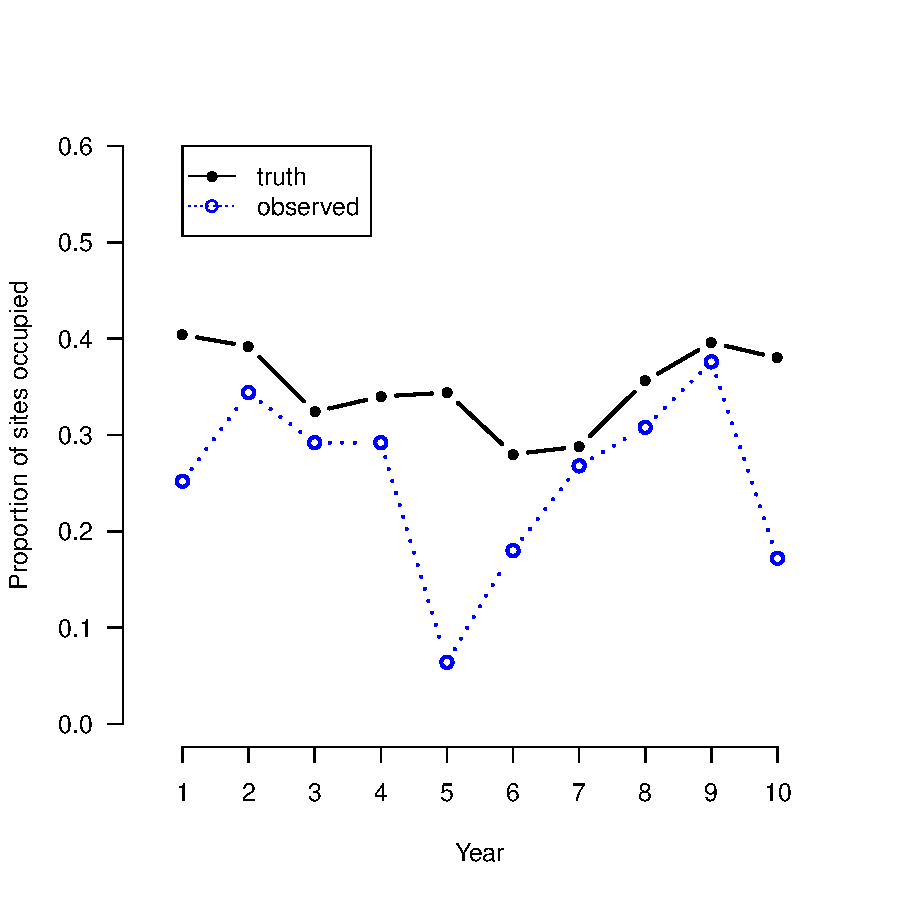
\includegraphics[width=4in,height=4in]{colext-sim.pdf}
\caption{Summary of the multi-year occupancy data set generated.}
\label{fig:sim}
\end{figure}


To analyze this data set with a dynamic occupancy model in
\textbf{unmarked}, we first load the package.

\begin{Schunk}
\begin{Sinput}
> library(unmarked)
\end{Sinput}
\end{Schunk}

Next, we reformat the detection/non-detection data from a 3-dimensional
array (as generated) into a 2-dimensional matrix with M rows.
That is, we put the annual tables of data (the slices of the former
3-D array) sideways to produce a ``wide'' layout of the data.

\begin{small}
\begin{Schunk}
\begin{Sinput}
> yy <- matrix(y, M, J*T)
\end{Sinput}
\end{Schunk}
\end{small}


Next, we create a matrix indicating the year each site was surveyed.

\begin{small}
\begin{Schunk}
\begin{Sinput}
> year <- matrix(c('01','02','03','04','05','06','07','08','09','10'),
                nrow(yy), T, byrow=TRUE)
\end{Sinput}
\end{Schunk}
\end{small}

To organize the data in the format required by \emph{colext}, we make
use of the function \emph{unmarkedMultFrame}. The only required
arguments are \emph{y}, the detection/non-detection data, and
\emph{numPrimary}, the number of seasons. The three types of
covariates described earlier can also be supplied using the arguments
\emph{siteCovs}, \emph{yearlySiteCovs}, and \emph{obsCovs}. In this case,
we only make use of the second type, which must have M rows and T
columns.

\begin{small}

\begin{Schunk}
\begin{Sinput}
> simUMF <- unmarkedMultFrame(
     y = yy,
     yearlySiteCovs = list(year = year),
     numPrimary=T)
> summary(simUMF)
\end{Sinput}
\begin{Soutput}
unmarkedFrame Object

250 sites
Maximum number of observations per site: 30 
Mean number of observations per site: 30 
Number of primary survey periods: 10 
Number of secondary survey periods: 3 
Sites with at least one detection: 195 

Tabulation of y observations:
   0    1 <NA> 
6430 1070    0 

Yearly-site-level covariates:
      year     
 01     : 250  
 02     : 250  
 03     : 250  
 04     : 250  
 05     : 250  
 06     : 250  
 (Other):1000  
\end{Soutput}
\end{Schunk}
\end{small}



\subsection{Model fitting}
We are ready to fit a few dynamic occupancy models.
We will fit a model with constant values for all parameters and
another with full time-dependence for colonization, extinction and
detection probability. We also time the calculations.

\begin{small}

\begin{Schunk}
\begin{Sinput}
> # Model with all constant parameters
> m0 <- colext(psiformula= ~1, gammaformula = ~ 1, epsilonformula = ~ 1,
              pformula = ~ 1, data = simUMF, method="BFGS")
\end{Sinput}
\end{Schunk}

\begin{Schunk}
\begin{Sinput}
> summary(m0)
\end{Sinput}
\begin{Soutput}
Call:
colext(psiformula = ~1, gammaformula = ~1, epsilonformula = ~1, 
    pformula = ~1, data = simUMF, method = "BFGS")

Initial (logit-scale):
 Estimate    SE     z  P(>|z|)
   -0.813 0.158 -5.16 2.46e-07

Colonization (logit-scale):
 Estimate     SE   z   P(>|z|)
    -1.77 0.0807 -22 2.75e-107

Extinction (logit-scale):
 Estimate    SE     z  P(>|z|)
    -0.59 0.102 -5.79 7.04e-09

Detection (logit-scale):
 Estimate     SE     z P(>|z|)
  -0.0837 0.0562 -1.49   0.137

AIC: 4972.597 
Number of sites: 250
optim convergence code: 0
optim iterations: 27 
Bootstrap iterations: 0 
\end{Soutput}
\end{Schunk}

\end{small}


The computation time was only a few seconds.
Note that all parameters were estimated on the logit scale. To
back-transform to the original scale, we can simply use the
inverse-logit function, named \emph{plogis} in R.

\begin{small}

\begin{Schunk}
\begin{Sinput}
> plogis(-0.813)
\end{Sinput}
\begin{Soutput}
[1] 0.3072516
\end{Soutput}
\end{Schunk}
\end{small}


Alternatively, we can use \emph{backTransform}, which
computes standard errors using the delta method. Confidence intervals
are also easily obtained using the function \emph{confint}.
We first remind ourselves of the names of parameters, which can all be
used as arguments for these functions.


\begin{small}

\begin{Schunk}
\begin{Sinput}
> names(m0)
\end{Sinput}
\begin{Soutput}
[1] "psi" "col" "ext" "det"
\end{Soutput}
\begin{Sinput}
> backTransform(m0, type="psi")
\end{Sinput}
\begin{Soutput}
Backtransformed linear combination(s) of Initial estimate(s)

 Estimate     SE LinComb (Intercept)
    0.307 0.0335  -0.813           1

Transformation: logistic 
\end{Soutput}
\begin{Sinput}
> confint(backTransform(m0, type="psi"))
\end{Sinput}
\begin{Soutput}
     0.025     0.975
 0.2457313 0.3765804
\end{Soutput}
\end{Schunk}
\end{small}


Next, we fit the dynamic occupancy model with full year-dependence in
the parameters describing occupancy dynamics and also in detection.
This is the same model under which we generated the data set, so we
would expect accurate estimates.

By default in R, a factor such as year in this analysis, is a
parameterized in terms of an intercept and effects representing
differences. This would mean that the parameter for the first year is
the intercept  and the effects would denote the differences between
the parameter  values in all other years, relative to the parameter
value in the first year, which serves as a reference level.
This treatment or effects parameterization is useful for testing for
differences. For simple presentation, a means parameterization is more
practical. It can be specified by adding a -1 to the formula for the
time-dependent parameters.

\begin{small}

\begin{Schunk}
\begin{Sinput}
> m1 <- colext(psiformula = ~1,   # First-year occupancy
     gammaformula = ~ year-1,    # Colonization
     epsilonformula = ~ year-1,  # Extinction
     pformula = ~ year-1,        # Detection
     data = simUMF)
\end{Sinput}
\end{Schunk}
\begin{Schunk}
\begin{Sinput}
> m1
\end{Sinput}
\begin{Soutput}
Call:
colext(psiformula = ~1, gammaformula = ~year - 1, epsilonformula = ~year - 
    1, pformula = ~year - 1, data = simUMF)

Initial:
 Estimate    SE      z P(>|z|)
   -0.273 0.302 -0.906   0.365

Colonization:
       Estimate    SE     z  P(>|z|)
year01    -2.08 0.951 -2.19 2.86e-02
year02    -2.18 0.365 -5.96 2.52e-09
year03    -1.98 0.274 -7.23 4.88e-13
year04    -2.32 0.678 -3.42 6.37e-04
year05    -1.89 0.478 -3.95 7.78e-05
year06    -1.76 0.294 -5.97 2.44e-09
year07    -1.55 0.230 -6.73 1.75e-11
year08    -1.43 0.228 -6.29 3.19e-10
year09    -2.35 0.470 -5.00 5.64e-07

Extinction:
       Estimate    SE      z  P(>|z|)
year01  -1.4209 0.418 -3.401 6.72e-04
year02  -0.4808 0.239 -2.009 4.45e-02
year03  -1.2606 0.366 -3.440 5.83e-04
year04  -0.0907 0.650 -0.139 8.89e-01
year05  -0.6456 0.599 -1.078 2.81e-01
year06  -0.9586 0.378 -2.539 1.11e-02
year07  -1.2279 0.365 -3.362 7.74e-04
year08  -1.1894 0.292 -4.076 4.58e-05
year09  -0.6292 0.635 -0.991 3.22e-01

Detection:
       Estimate    SE      z  P(>|z|)
year01  -1.0824 0.244 -4.434 9.26e-06
year02  -0.2232 0.148 -1.508 1.32e-01
year03   0.2951 0.154  1.918 5.52e-02
year04   0.0662 0.161  0.412 6.81e-01
year05  -2.0396 0.433 -4.706 2.52e-06
year06  -0.6982 0.232 -3.005 2.66e-03
year07   0.2413 0.165  1.466 1.43e-01
year08   0.0847 0.155  0.548 5.84e-01
year09   0.6052 0.140  4.338 1.44e-05
year10  -1.1699 0.306 -3.828 1.29e-04

AIC: 4779.172 
\end{Soutput}
\end{Schunk}
\end{small}




\subsection{Manipulating results: prediction and plotting}

Again, all estimates are shown on the logit-scale. Back-transforming
estimates when covariates, such as year, are present involves an
extra step. Specifically, we need to tell \textbf{unmarked} the values
of our covariate
at which we want an estimate. This can be done using
\emph{backTransform} in combination with \emph{linearComb}, although
it can be easier to use \emph{predict}. \emph{predict} allows the user
to supply a data.frame in which each row represents a combination of
covariate values of interest. Below, we create data.frames called
\emph{nd} with each row representing a year.
Then we request yearly estimates of the probability of extinction,
colonization and detection,
and compare them to ``truth'', i.e., the values with which we
simulated the data set. Note that there are T-1 extinction and
colonization parameters in this case, so we do not need to include
year `10' in \emph{nd}.

\begin{small}

\begin{Schunk}
\begin{Sinput}
> nd <- data.frame(year=c('01','02','03','04','05','06','07','08','09'))
> E.ext <- predict(m1, type='ext', newdata=nd)
> E.col <- predict(m1, type='col', newdata=nd)
> nd <- data.frame(year=c('01','02','03','04','05','06','07','08','09','10'))
> E.det <- predict(m1, type='det', newdata=nd)
\end{Sinput}
\end{Schunk}
\end{small}


Predict returns the predictions along with standard errors and
confidence intervals. These can be used to create plots. The
\emph{with} function is used to simplify the process of requesting the
columns of data.frame returned by \emph{predict}.


\begin{small}

\begin{Schunk}
\begin{Sinput}
> op <- par(mfrow=c(3,1), mai=c(0.6, 0.6, 0.1, 0.1))
> with(E.ext, {   # Plot for extinction probability
   plot(1:9, Predicted, pch=1, xaxt='n', xlab='Year',
     ylab=expression(paste('Extinction probability ( ', epsilon, ' )')),
     ylim=c(0,1), col=4)
   axis(1, at=1:9, labels=nd$year[1:9])
   arrows(1:9, lower, 1:9, upper, code=3, angle=90, length=0.03, col=4)
   points((1:9)-0.1, 1-phi, col=1, lwd = 1, pch=16)
   legend(7, 1, c('Parameter', 'Estimate'), col=c(1,4), pch=c(16, 1),
          cex=0.8)
   })
> with(E.col, {	# Plot for colonization probability
   plot(1:9, Predicted, pch=1, xaxt='n', xlab='Year',
     ylab=expression(paste('Colonization probability ( ', gamma, ' )')),
     ylim=c(0,1), col=4)
   axis(1, at=1:9, labels=nd$year[1:9])
   arrows(1:9, lower, 1:9, upper, code=3, angle=90, length=0.03, col=4)
   points((1:9)-0.1, gamma, col=1, lwd = 1, pch=16)
   legend(7, 1, c('Parameter', 'Estimate'), col=c(1,4), pch=c(16, 1),
          cex=0.8)
   })
> with(E.det, {   # Plot for detection probability: note 10 years
   plot(1:10, Predicted, pch=1, xaxt='n', xlab='Year',
     ylab=expression(paste('Detection probability ( ', p, ' )')),
     ylim=c(0,1), col=4)
   axis(1, at=1:10, labels=nd$year)
   arrows(1:10, lower, 1:10, upper, code=3, angle=90, length=0.03, col=4)
   points((1:10)-0.1, p, col=1, lwd = 1, pch=16)
   legend(7.5, 1, c('Parameter','Estimate'), col=c(1,4), pch=c(16, 1),
          cex=0.8)
   })
> par(op)
\end{Sinput}
\end{Schunk}

\end{small}




\begin{figure}
  \centering
  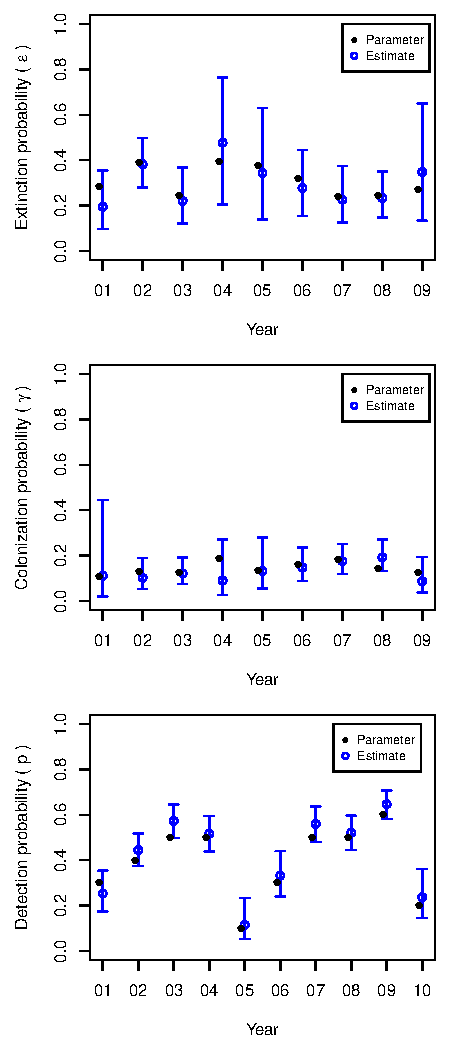
\includegraphics[width=3in,height=7in]{colext-yearlysim.pdf}
  \caption{Yearly estimates of $\epsilon$, $\gamma$ and $p$.}
  \label{fig:yearlysim}
\end{figure}

Figure~\ref{fig:yearlysim} shows that the 95\% confidence intervals
include the true parameter values, and the point estimates are not too
far off.


\subsection{Derived parameters}

Estimates of occupancy probability in years $T>1$ must be derived from the
estimates of first-year occupancy and the two parameters governing the
dynamics, extinction/survival and colonization.
\textbf{unmarked} does this automatically in two ways. First, the
population-level estimates of occupancy probability
$\psi_t = \psi_{t-1}\phi_{t-1} + (1-\phi_{t-1})\gamma$ are calculated
and stored in the slot named \emph{projected}. Slots can be accessed
using the @ operator, e.g. fm@projected.
In some cases, interest may lie in making
inference about the proportion of the sampled sites that are occupied,
rather than the entire population of sites. These estimates are
contained in the \emph{smoothed} slot of the fitted model. Thus, the
\emph{projected} values are estimates of population parameters, and
the \emph{smoothed} estimates are of the finite-sample
quantities. Discussions of the differences can be found in Weir et
al. (2009).

Bootstrap methods can be used to compute standard errors of derived
parameter estimates. Here we employ a non-parametric bootstrap to obtain
standard errors of the smoothed estimates of occupancy probability
during each year.

\begin{small}
\begin{Schunk}
\begin{Sinput}
> m1 <- nonparboot(m1, B = 100)
\end{Sinput}
\end{Schunk}
\begin{Schunk}
\begin{Sinput}
> cbind(psi=psi, smoothed=smoothed(m1)[2,], SE=m1@smoothed.mean.bsse[2,])
\end{Sinput}
\end{Schunk}
\end{small}


In practice, B should be much higher, possibly $>$ 1000 for complex
models .

Another derived parameters of interest is turnover probability

\[
\tau_t = \frac{\gamma_{t-1}(1-\psi_{t-1})}{\gamma_{t-1}(1-\psi_{t-1})
  + \phi_{t-1}\psi_{t-1}}
\]

The following function returns these estimates.

\begin{small}

\begin{Schunk}
\begin{Sinput}
> turnover <- function(fm) {
     psi.hat <- plogis(coef(fm, type="psi"))
     if(length(psi.hat) > 1)
         stop("this function only works if psi is scalar")
     T <- getData(fm)@numPrimary
     tau.hat <- numeric(T-1)
     gamma.hat <- plogis(coef(fm, type="col"))
     phi.hat <- 1 - plogis(coef(fm, type="ext"))
     if(length(gamma.hat) != T-1 | length(phi.hat) != T-1)
         stop("this function only works if gamma and phi T-1 vectors")
     for(t in 2:T) {
         psi.hat[t] <- psi.hat[t-1]*phi.hat[t-1] +
             (1-psi.hat[t-1])*gamma.hat[t-1]
         tau.hat[t-1] <- gamma.hat[t-1]*(1-psi.hat[t-1]) / psi.hat[t-1]
         }
     return(tau.hat)
     }
\end{Sinput}
\end{Schunk}
\end{small}



The bootstrap again offers a means of estimating variance. Here we
show how to generate 95\% confidence intervals for the turnover
estimates using the parametric bootstrap.


\begin{small}


\begin{Schunk}
\begin{Sinput}
> pb <- parboot(m1, statistic=turnover, nsim=2)
> turnCI <- cbind(pb@t0,
     t(apply(pb@t.star, 2, quantile, probs=c(0.025, 0.975))))
> colnames(turnCI) <- c("tau", "lower", "upper")
\end{Sinput}
\end{Schunk}
\begin{Schunk}
\begin{Sinput}
> turnCI
\end{Sinput}
\begin{Soutput}
          tau     lower     upper
t*1 0.1457961 0.2920256 0.5515986
t*2 0.1460339 0.1110656 0.1639632
t*3 0.2648988 0.2635840 0.3215506
t*4 0.1840518 0.2560206 0.6640515
t*5 0.4353955 0.1600642 0.9629842
t*6 0.4353175 0.3364786 0.6813287
t*7 0.4233780 0.4337405 0.6141042
t*8 0.3566357 0.3185164 0.3319792
t*9 0.1340253 0.1030345 0.1956252
\end{Soutput}
\end{Schunk}


\end{small}


Which bootstrap method is most appropriate for variance estimation?
For detailed distinctions between the
non-parametric and the parametric bootstrap, see Davison and Hinkley
(1997). We note simply that the parametric bootstrap resamples from
the fitted model, and thus the
measures of uncertainty are purely
functions of the distributions assumed by the model. Non-parametric
bootstrap samples, in contrast, are obtained by resampling the
data, not the model, and thus are not necessarily affected by the
variance formulas of the model's distributions.



\subsection{Goodness-of-fit}


In addition to estimating the variance of an estimate, the parametric
bootstrap can be used to assess goodness-of-fit. For this purpose, a
fit-statistic, i.e. one that compares
observed and expected values, is evaluated using the original fitted
model, and numerous other models fitted to simulated datasets. The
simulation yields an approximation of
the distribution of the fit-statistic, and a \emph{P}-value
can be computed as the proportion of simulated values greater than the
observed value.

Hosmer et al. (1997) found that a $\chi^2$ statistic performed
reasonably well in assessing lack of fit for logistic regression
models. We know of no studies formally
evaluating the performance of various fit-statistics for dynamic
occupancy models, so this approach should be
considered experimental. Fit-statistics applied to aggregated
encounter histories offer an alternative approach (MacKenzie and
Bailey 2004), but are difficult to implement when J*T is high and
missing values or continuous covariates are present.


\begin{small}

\begin{Schunk}
\begin{Sinput}
> chisq <- function(fm) {
     umf <- getData(fm)
     y <- getY(umf)
     sr <- fm@sitesRemoved
     if(length(sr)>0)
         y <- y[-sr,,drop=FALSE]
     fv <- fitted(fm, na.rm=TRUE)
     y[is.na(fv)] <- NA
     sum((y-fv)^2/(fv*(1-fv)))
     }
> pb.gof <- parboot(m0, statistic=chisq, nsim=100)
\end{Sinput}
\end{Schunk}

%<<eval=false,gof,echo=false,fig=true,include=false,width=6,height=6>>=
%plot(pb.gof, xlab=expression(chi^2), main="", col=gray(0.95))
%@
\end{small}


\begin{figure}[!h]
\centering
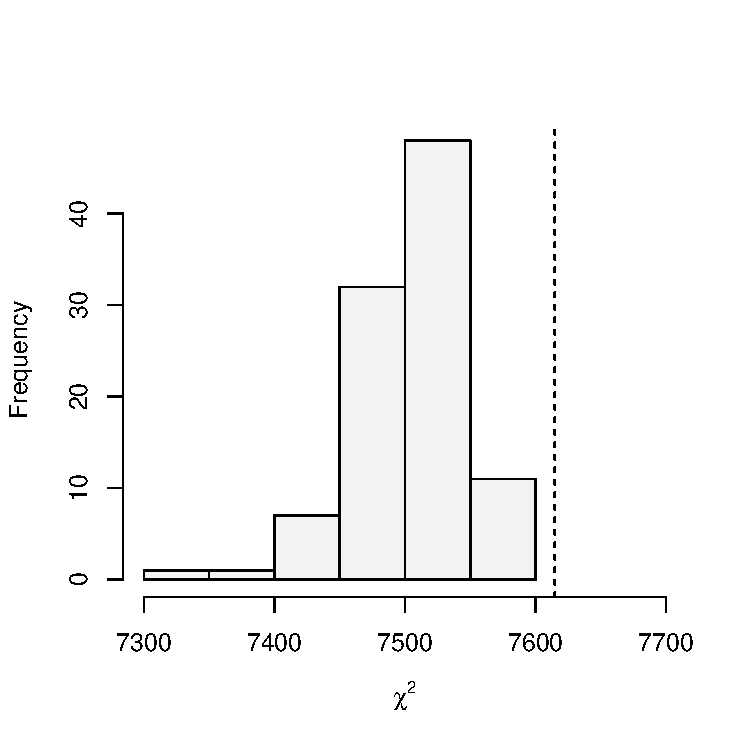
\includegraphics[width=4in,height=4in]{colext-gof.pdf}
\caption{Goodness-of-fit}
\label{fig:gof}
\end{figure}

Figure~\ref{fig:gof} indicates that, as expected, the constant
parameter model does not fit the data well.



\section{Dynamic occupancy models for crossbill data from the Swiss MHB}

\subsection{The crossbill data set}
The crossbill data are in a comma-delimited text file called
`crossbill.csv'.
This file contains the results of nine years of surveys (1999--2007)
for the European crossbill (\emph{Loxia curvirostra}),
a pine-seed eating finch, in 267 1-km$^2$ sample quadrats in Switzerland.
Quadrats are surveyed annually as part of the Swiss breeding bird
survey MHB (Schmid et al. 2004).
They are laid out as a grid over Switzerland and surveyed 2 or 3 times
every breeding season (mid-April to late June)
by experienced field ornithologists along a haphazard survey route of
length 1--9 km (average 5 km).
High-elevation sites are only surveyed twice per breeding season.



\subsection{Importing, formatting, and summarizing data}
We import the data into an open R workspace using a standard method,
and display the column names.

\begin{small}

\begin{Schunk}
\begin{Sinput}
> crossbill <- read.csv(system.file("csv", "crossbill.csv",
     package="unmarked"), header=TRUE)
> colnames(crossbill)
\end{Sinput}
\begin{Soutput}
 [1] "id"      "ele"     "forest"  "surveys" "det991"  "det992" 
 [7] "det993"  "det001"  "det002"  "det003"  "det011"  "det012" 
[13] "det013"  "det021"  "det022"  "det023"  "det031"  "det032" 
[19] "det033"  "det041"  "det042"  "det043"  "det051"  "det052" 
[25] "det053"  "det061"  "det062"  "det063"  "det071"  "det072" 
[31] "det073"  "date991" "date992" "date993" "date001" "date002"
[37] "date003" "date011" "date012" "date013" "date021" "date022"
[43] "date023" "date031" "date032" "date033" "date041" "date042"
[49] "date043" "date051" "date052" "date053" "date061" "date062"
[55] "date063" "date071" "date072" "date073"
\end{Soutput}
\end{Schunk}
\end{small}


We have three covariates that vary by site: median elevation of the
quadrat (ele, in metres), forest cover of the quadrat (forest, in
percent) and the number of surveys per season (i.e., 2 or 3,
surveys).
These are called site covariates, because they vary by sites only.
The 27 columns entitled ``det991''--``det073'' contain the crossbill
detection/nondetection data during all surveys over the 9 years.
They contain a 1 when at least one crossbill was recorded during a
survey and a 0 otherwise.
NAs indicate surveys that did not take place, either because a site is
high-elevation and has no third survey or because it failed to be
surveyed altogether in a year.
The final 27 columns entitled ``date991'' -- ``date073'' give the Julian
date of each survey.
They represent a `survey-covariate' or `observation covariate'.
We note that the paper by Royle and K\'{e}ry (2007) used a subset of this
data set.

AIC-based model selection (see section 4.4.) requires
that all models are fit to the same data.
\textbf{unmarked} removes missing data in a context specific way. For
missing siteCovs, the entire row of data must be removed. However, for
missing \emph{yearlySiteCovs} or \emph{obsCovs}, only the
corresponding observation
are removed. Thus, if \textbf{unmarked} removes different observations
from different models, the models cannot be compared using AIC. A way
around this is to remove the detection data corresponding to
missing covariates before fitting the models.
The crossbill data have missing dates and so we remove the associated
detection/non-detection data.


\begin{Schunk}
\begin{Sinput}
> DATE <- as.matrix(crossbill[,32:58])
> y.cross <- as.matrix(crossbill[,5:31])
> y.cross[is.na(DATE) != is.na(y.cross)] <- NA
\end{Sinput}
\end{Schunk}

In addition, continuous covariates should be transformed in a way
that brings their values close to zero in order to improve
or even enable numerical convergence of the maximum-likelihood routine.
We do this ``by hand'' and note that we could also have used the R
function \emph{scale}. We subtract the mean and divide by the standard
deviation.

\begin{small}

\begin{Schunk}
\begin{Sinput}
> sd.DATE <- sd(c(DATE), na.rm=TRUE)
> mean.DATE <- mean(DATE, na.rm=TRUE)
> DATE <- (DATE - mean.DATE) / sd.DATE
\end{Sinput}
\end{Schunk}
\end{small}

Before we can fit occupancy models, we need to format this data set
appropriately.


\begin{small}

\begin{Schunk}
\begin{Sinput}
> years <- as.character(1999:2007)
> years <- matrix(years, nrow(crossbill), 9, byrow=TRUE)
> umf <- unmarkedMultFrame(y=crossbill[,5:31],
     siteCovs=crossbill[,2:3], yearlySiteCovs=list(year=years),
     obsCovs=list(date=DATE),
     numPrimary=9)
\end{Sinput}
\end{Schunk}
\end{small}



\subsection{Model fitting}
We fit a series of models that represent different hypotheses about
the colonization-extinction dynamics of Swiss crossbills
at a spatial scale of 1 km$^2$.
We fit year effects on colonization and extinction in the means
parameterization,
but for detection probability, we choose an effects parameterization.
The latter is more useful for getting predictions in the presence of
other explanatory variables for that parameter.
For model fm5 with more complex covariate relationships, we use as
starting values for the optimization routine
the solution from a ``neighbouring'' model with slightly less
complexity, model fm4.
Wise choice of starting values can be decisive for success or failure
of maximum likelihood estimation.


\begin{small}

\begin{Schunk}
\begin{Sinput}
> # A model with constant parameters
> fm0 <- colext(~1, ~1, ~1, ~1, umf)
\end{Sinput}
\end{Schunk}
\begin{Schunk}
\begin{Sinput}
> # Like fm0, but with year-dependent detection
> fm1 <- colext(~1, ~1, ~1, ~year, umf)
\end{Sinput}
\end{Schunk}
\begin{Schunk}
\begin{Sinput}
> # Like fm0, but with year-dependent colonization and extinction
> fm2 <- colext(~1, ~year-1, ~year-1, ~1, umf)
\end{Sinput}
\end{Schunk}
\begin{Schunk}
\begin{Sinput}
> # A fully time-dependent model
> fm3 <- colext(~1, ~year-1, ~year-1, ~year, umf)
\end{Sinput}
\end{Schunk}
\begin{Schunk}
\begin{Sinput}
> # Like fm3 with forest-dependence of 1st-year occupancy
> fm4 <- colext(~forest, ~year-1, ~year-1, ~year, umf)
\end{Sinput}
\end{Schunk}
\begin{Schunk}
\begin{Sinput}
> # Like fm4 with date- and year-dependence of detection
> fm5 <- colext(~forest, ~year-1, ~year-1, ~year + date + I(date^2),
               umf, starts=c(coef(fm4), 0, 0))
\end{Sinput}
\end{Schunk}
\begin{Schunk}
\begin{Sinput}
> # Same as fm5, but with detection in addition depending on forest cover
> fm6 <- colext(~forest, ~year-1, ~year-1, ~year + date + I(date^2) +
               forest, umf)
\end{Sinput}
\end{Schunk}
\end{small}




\subsection{Model selection}
We can compare models using the Akaike information criterion
($AIC$).
Note that \textbf{unmarked} yields $AIC$, not $AIC_c$
because the latter would require the sample size,
which is not really known for
hierarchical models such as the dynamic occupancy model.

Model selection and model-averaged prediction in \textbf{unmarked}
require that we create a list of models using \emph{fitList}.
This function organizes models and conducts a series of tests to
ensure that the models were fit to the same data.

\begin{small}

%<<eval=true>>=
%models <- fitList('psi(.)gam(.)eps(.)p(.)'    = fm0,
%                   'psi(.)gam(.)eps(.)p(Y)'    = fm1,
%                   'psi(.)gam(Y)eps(Y)p(.)'    = fm2,
%                   'psi(.)gam(Y)eps(Y)p(Y)'    = fm3,
%                   'psi(F)gam(Y)eps(Y)p(Y)'    = fm4,
%                   'psi(F)gam(Y)eps(Y)p(YD2)'  = fm5,
%                   'psi(F)gam(Y)eps(Y)p(YD2F)' = fm6)
%ms <- modSel(models)
%ms
%@

\begin{Schunk}
\begin{Sinput}
> models <- fitList('psi(.)gam(.)eps(.)p(.)'    = fm0,
                    'psi(.)gam(.)eps(.)p(Y)'    = fm1,
                    'psi(.)gam(Y)eps(Y)p(.)'    = fm2,
                    'psi(.)gam(Y)eps(Y)p(Y)'    = fm3,
                    'psi(F)gam(Y)eps(Y)p(Y)'    = fm4,
                    'psi(F)gam(Y)eps(Y)p(YD2)'  = fm5,
                    'psi(F)gam(Y)eps(Y)p(YD2F)' = fm6)
> ms <- modSel(models)
> ms
\end{Sinput}
\begin{Soutput}
                          nPars     AIC  delta   AICwt cumltvWt
psi(F)gam(Y)eps(Y)p(YD2F)    30 5000.85   0.00 1.0e+00     1.00
psi(F)gam(Y)eps(Y)p(YD2)     29 5077.03  76.19 2.9e-17     1.00
psi(F)gam(Y)eps(Y)p(Y)       27 5099.15  98.31 4.5e-22     1.00
psi(.)gam(.)eps(.)p(Y)       12 5115.80 114.95 1.1e-25     1.00
psi(.)gam(Y)eps(Y)p(Y)       26 5131.34 130.49 4.6e-29     1.00
psi(.)gam(Y)eps(Y)p(.)       18 5173.21 172.36 3.7e-38     1.00
psi(.)gam(.)eps(.)p(.)        4 5197.44 196.60 2.0e-43     1.00
\end{Soutput}
\end{Schunk}

\end{small}



One model has overwhelming support, so we can base inference on that
one alone. Before doing so, we point out how to extract coefficients
from a \emph{fitList} object, and convert the results to a
\emph{data.frame}, which could be exported from R.

\begin{small}

%<<eval=false>>=
%coef(ms)                            # Estimates only
%SE(ms)                              # Standard errors only
%toExport <- as(ms, "data.frame")    # Everything
%@

\begin{Schunk}
\begin{Sinput}
> coef(ms)                            # Estimates only
> SE(ms)                              # Standard errors only
> toExport <- as(ms, "data.frame")    # Everything
\end{Sinput}
\end{Schunk}


\end{small}



\subsection{Manipulating results: Prediction and plotting}
Fitted models can be used to predict expected outcomes when given new
data. For example, one could ask ``how many crossbills would you
expect to find in a quadrat with 50\% forest cover?'' Prediction also
offers a way of
presenting the results of an analysis. We illustrate by plotting the
predictions of $\psi$ and $p$ over the range of covariate values studied.
Note that because we standardized date, we need to transform it back
to its original scale after obtaining predictions on the
standardized scale.


\begin{small}

\begin{Schunk}
\begin{Sinput}
> op <- par(mfrow=c(1,2), mai=c(0.8,0.8,0.1,0.1))
> nd <- data.frame(forest=seq(0, 100, length=50))
> E.psi <- predict(fm6, type="psi", newdata=nd, appendData=TRUE)
> with(E.psi, {
     plot(forest, Predicted, ylim=c(0,1), type="l",
          xlab="Percent cover of forest",
          ylab=expression(hat(psi)), cex.lab=0.8, cex.axis=0.8)
     lines(forest, Predicted+1.96*SE, col=gray(0.7))
     lines(forest, Predicted-1.96*SE, col=gray(0.7))
     })
> nd <- data.frame(date=seq(-2, 2, length=50),
                  year=factor("2005", levels=c(unique(years))),
                  forest=50)
> E.p <- predict(fm6, type="det", newdata=nd, appendData=TRUE)
> E.p$dateOrig <- E.p$date*sd.DATE + mean.DATE
> with(E.p, {
     plot(dateOrig, Predicted, ylim=c(0,1), type="l",
          xlab="Julian date", ylab=expression( italic(p) ),
          cex.lab=0.8, cex.axis=0.8)
     lines(dateOrig, Predicted+1.96*SE, col=gray(0.7))
     lines(dateOrig, Predicted-1.96*SE, col=gray(0.7))
     })
> par(op)
\end{Sinput}
\end{Schunk}

\end{small}


\begin{figure}[!h]
\centering
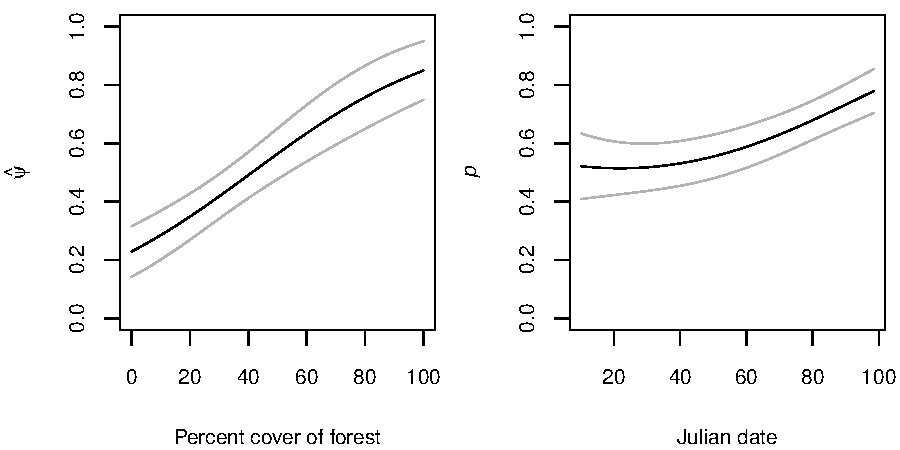
\includegraphics[width=6in,height=3in]{colext-cov.pdf}
\caption{Covariates}
\label{fig:cov}
\end{figure}






\section*{Acknowledgements}
Special thanks goes to Ian Fiske, the author of \emph{colext} and the
original developer of \textbf{unmarked}. Andy Royle provided the
initial funding and support for the package. The questions of many
people on the users' list motivated the writing of this document.



\newpage

\section*{References}
\newcommand{\rf}{\vskip .1in\par\sloppy\hangindent=1pc\hangafter=1
                  \noindent}

\rf Davison, A.C and D.V. Hinkley. 1997. \emph{Bootstrap Methods and Their
Application}, first ed. Cambridge University Press.

\rf Dorazio, R.M., and Royle, J.A. 2005. Estimating size and
composition of biological communities by modeling the occurrence of
species. Journal of the American Statistical Association 100:
389--398.

\rf Dorazio, R.M., K\'{e}ry, M., Royle, J.A., and Plattner,
M. 2010. Models for inference in dynamic metacommunity
systems. Ecology 91: 2466--2475.

\rf Hanski, I. 1998. Metapopulation dynamics. Nature 396: 41--49.

\rf Hosmer, D.W., T. Hosmer, S. le Cressie, and S. Lemeshow. 1997. A
comparision of goodness-of-fit tests for the logistic
regression model. Statistics in Medicine 16:965--980.

\rf K\'{e}ry, M. 2010. \emph{Introduction to WinBUGS for
  Ecologists. A Bayesian approach to regression, ANOVA, mixed
  models and related analyses}. Academic Press, Burlington, MA.

\rf K\'{e}ry, M., Royle, J.A., Plattner, M, and Dorazio,
R.M. 2009. Species richness and occupancy estimation in communities
subject to temporary emigration. Ecology 90: 1279--1290.

\rf K\'{e}ry, M., and Schaub, M. 2011. \emph{Bayesian population
  analysis using WinBUGS}. Academic Press, Burlington. (due December
2011)

\rf K\'{e}ry, M., and Schmidt, B.R. 2008. Imperfect detection and its
consequences for monitoring for conservation. Community Ecology 9:
207--216.

\rf MacKenzie, D.I and L. Bailey. 2004. Assessing the fit of
site-occupancy models. Journal of Agricultural, Biological, and
Environmental Statistics 9:300--318.

\rf MacKenzie, D.I., Nichols, J.D., Hines, J.E., Knutson, M.G., and
Franklin, A.B. 2003. Estimating site occupancy, colonization, and
local extinction when a species is detected imperfectly. Ecology 84:
2200--2207.

\rf MacKenzie, D.I., Nichols, J.D., Lachman, G.B., Droege, S., Royle,
J.A., and Langtimm, C.A. 2002. Estimating site occupancy rates when
detection probability rates are less than one. Ecology 83:
2248--2255.

\rf MacKenzie, D.I., Nichols, J.D., Seamans, M.E., and Gutierrez,
R.J. 2009. Modeling species occurrence dynamics with multiple states
and imperfect detection. Ecology 90: 823--835.

\rf McCullagh, P., and Nelder, J.A. 1989. \emph{Generalized linear
  models}. Chapman and Hall.

\rf Miller, D.A., Nichols, J.D., McClintock, B.T., Grant, E.H.C.,
Bailey, L.L., and Weir, L. 2011. Improving occupancy estimation when
two types of observational errors occur: non-detection and species
misidentification. Ecology, in press.

\rf Moilanen, A. 2002. Implications of empirical data quality to
metapopulation model parameter estimation and application. Oikos 96:
516--530.

\rf Nichols, J.D., Hines, J.E., MacKenzie, D.I., Seamans, M.E., and
Gutierrez, R.J. 2007. Occupancy estimation and modeling with multiple
states and state uncertainty. Ecology 88: 1395--1400.

\rf Royle, J.A., Dorazio, R.M. 2008. \emph{Hierarchical modeling and
  inference in ecology: The analysis of data from populations,
  metapopulations, and communities}. Academic Press, San Diego.

\rf Royle, J.A.,  and K\'{e}ry, M. 2007. A Bayesian state-space
formulation of dynamic occupancy models. Ecology 88: 1813--1823.

\rf Royle, J.A., and Link, W.A., 2005. A general class of multinomial
mixture models for anuran calling survey data. Ecology 86:
2505--2512.

\rf Royle, J.A., and Link, W.A., 2006. Generalized site occupancy
models allowing for false positive and false negative errors. Ecology
87: 835--841.

\rf Royle, J.A., and Nichols, J.D. 2003. Estimating abundance from
repeated presence-absence data or point counts. Ecology 84, 777--790.

\rf Schmid, H., Zbinden, N., and Keller,
V. 2004. \emph{\"{U}berwachung der Bestandsentwicklung h\"{a}ufiger
  Brutv\"{o}gel in der Schweiz}. Swiss Ornithological Institute,
Sempach, Switzerland.

\rf Tyre, A.J., Tenhumberg, B., Field, S.A., Niejalke, D., Parris, K.,
and Possingham, H.P. 2003. Improving precision and reducing bias in
biological surveys: estimating false-negative error rates. Ecological
Applications 13, 1790--1801.

\rf Weir, L., I.J. Fiske, and J.A. Royle. 2009. Trends in anuran
occupancy from northeastern states of the North American Amphibian
Monitoring Program. Herpetological Conservation and Biology
4:389--402.


\end{document}
